%%% Relatorio Tecnico - Atividade 6 - UTFPR
%%% Detector de maximo e minimo em VHDL

\documentclass[12pt,a4paper, brazil]{article}

%%%%%%% INFORMACOES DO CABECALHO
\newcommand{\workingDate}{\textsc{\selectlanguage{portuguese}\today}}
\newcommand{\userName}{LRCO7A}
\newcommand{\institution}{UTFPR-AP}
\usepackage{researchdiary_png}

\usepackage{listings}
\usepackage{float}
\usepackage{placeins}
\usepackage{booktabs}

\lstdefinestyle{vhdl}{
    language=VHDL,
    basicstyle=\ttfamily\small,
    keywordstyle=\color{blue}\bfseries,
    commentstyle=\color{gray}\itshape,
    stringstyle=\color{red},
    numbers=left,
    numberstyle=\tiny\color{gray},
    numbersep=5pt,
    frame=single,
    breaklines=true,
    captionpos=b,
    tabsize=2,
    inputencoding=utf8,
    extendedchars=true,
    literate=
        {á}{{\'a}}1 {à}{{\`a}}1 {â}{{\^a}}1 {ã}{{\~a}}1
        {é}{{\'e}}1 {ê}{{\^e}}1
        {í}{{\'i}}1
        {ó}{{\'o}}1 {ô}{{\^o}}1 {õ}{{\~o}}1
        {ú}{{\'u}}1
        {ç}{{\c{c}}}1
        {Á}{{\'A}}1 {À}{{\`A}}1 {Â}{{\^A}}1 {Ã}{{\~A}}1
        {É}{{\'E}}1 {Ê}{{\^E}}1
        {Í}{{\'I}}1
        {Ó}{{\'O}}1 {Ô}{{\^O}}1 {Õ}{{\~O}}1
        {Ú}{{\'U}}1
        {Ç}{{\c{C}}}1
}

\begin{document}

\begin{center}
{\textbf {\huge Atividade Prática 6 -- Detector de Máximo e Mínimo}}\\[5mm]
{\large Pedro Lucas dos Reis Silva - RA: 2272040} \\[5mm]
{\large Lucas dos Reis Viana - RA: 2321645} \\[5mm]
\today\\[5mm]
\end{center}

% ============================================================
\section{Introdução}
% ============================================================

Esta atividade consiste na implementação, em VHDL, de um detector de valor mínimo e valor máximo para um conjunto de valores inteiros. O circuito recebe quatro entradas sem sinal de 2 bits e produz duas saídas: o menor valor encontrado e o maior valor encontrado.

Os conceitos novos utilizados foram:

\begin{itemize}
    \item \textbf{\texttt{package}}: arquivo separado usado para declarar tipos e subprogramas compartilhados pelo projeto;
    \item \textbf{\texttt{type}}: criação de um tipo de vetor de inteiros, utilizado para armazenar internamente os valores de entrada;
    \item \textbf{\texttt{procedure}}: subprograma responsável por percorrer o vetor e calcular mínimo e máximo;
    \item \textbf{\texttt{generic}}: parâmetros usados para definir a quantidade de entradas e a largura de bits dos valores.
\end{itemize}

% ============================================================
\section{Desenvolvimento}
% ============================================================

\subsection{Arquivos do Projeto}

O projeto foi dividido em dois arquivos VHDL:

\begin{itemize}
    \item \texttt{meupacote.vhd}: contém os tipos auxiliares e o procedimento \texttt{detector\_min\_max};
    \item \texttt{atividade6.vhd}: contém a entidade principal, as portas de entrada e saída e a chamada do procedimento.
\end{itemize}

A entidade principal é \texttt{atividade6}. Ela possui os genéricos \texttt{NUM\_INPUTS} e \texttt{NUM\_BITS}, com valores padrão iguais a 4 e 2, respectivamente. Assim, a versão implementada compara quatro valores de 2 bits.

\subsection{Entradas e Saídas}

As entradas e saídas externas foram declaradas como \texttt{std\_logic\_vector}, garantindo compatibilidade com o arquivo de formas de onda utilizado na simulação e com as atribuições de pinos do Quartus Prime. As portas são:

\begin{itemize}
    \item \texttt{e1}, \texttt{e2}, \texttt{e3}, \texttt{e4}: entradas de 2 bits;
    \item \texttt{saida\_min}: menor valor entre as quatro entradas;
    \item \texttt{saida\_max}: maior valor entre as quatro entradas.
\end{itemize}

Dentro da arquitetura, as entradas são convertidas para inteiros e armazenadas no sinal \texttt{x}, do tipo \texttt{int\_array}. Esse tipo foi declarado no pacote \texttt{meupacote}.

\subsection{Funcionamento Lógico}

O procedimento \texttt{detector\_min\_max} inicia o valor mínimo e o valor máximo com o primeiro elemento do vetor de entrada. Em seguida, um laço \texttt{for} percorre todos os elementos do vetor. Se o elemento atual for menor que o mínimo armazenado, o mínimo é atualizado. Se for maior que o máximo armazenado, o máximo é atualizado.

Na entidade principal, o procedimento é chamado dentro de um \texttt{process(x)}. Dessa forma, sempre que alguma entrada muda, o vetor interno \texttt{x} é atualizado e o procedimento recalcula as saídas.

Ao final, os valores calculados como inteiros são convertidos para \texttt{unsigned} e, em seguida, para \texttt{std\_logic\_vector}, formando as saídas \texttt{saida\_min} e \texttt{saida\_max}.

\subsection{Implementação na Placa DE10-Lite}

Na implementação física, as quatro entradas de 2 bits utilizam as chaves \texttt{SW0} a \texttt{SW7}. As saídas são apresentadas nos LEDs vermelhos: \texttt{LEDR0} e \texttt{LEDR1} indicam o menor valor, enquanto \texttt{LEDR8} e \texttt{LEDR9} indicam o maior valor. A Tabela~\ref{tab:pinagem} apresenta as atribuições definidas no arquivo \texttt{atividade6.qsf}. Todos os sinais utilizam o padrão elétrico \texttt{3.3-V LVTTL}.

\begin{table}[H]
\centering
\caption{Pinagem do detector de mínimo e máximo na placa DE10-Lite.}
\label{tab:pinagem}
\begin{tabular}{@{}llll@{}}
\toprule
\textbf{Recurso} & \textbf{Sinal VHDL} & \textbf{Função} & \textbf{Pino} \\
\midrule
\texttt{SW0}   & \texttt{e1(0)}          & bit 0 da entrada 1 & \texttt{PIN\_C10} \\
\texttt{SW1}   & \texttt{e1(1)}          & bit 1 da entrada 1 & \texttt{PIN\_C11} \\
\texttt{SW2}   & \texttt{e2(0)}          & bit 0 da entrada 2 & \texttt{PIN\_D12} \\
\texttt{SW3}   & \texttt{e2(1)}          & bit 1 da entrada 2 & \texttt{PIN\_C12} \\
\texttt{SW4}   & \texttt{e3(0)}          & bit 0 da entrada 3 & \texttt{PIN\_A12} \\
\texttt{SW5}   & \texttt{e3(1)}          & bit 1 da entrada 3 & \texttt{PIN\_B12} \\
\texttt{SW6}   & \texttt{e4(0)}          & bit 0 da entrada 4 & \texttt{PIN\_A13} \\
\texttt{SW7}   & \texttt{e4(1)}          & bit 1 da entrada 4 & \texttt{PIN\_A14} \\
\texttt{LEDR0} & \texttt{saida\_min(0)} & bit 0 do mínimo    & \texttt{PIN\_A8}  \\
\texttt{LEDR1} & \texttt{saida\_min(1)} & bit 1 do mínimo    & \texttt{PIN\_A9}  \\
\texttt{LEDR8} & \texttt{saida\_max(0)} & bit 0 do máximo    & \texttt{PIN\_A11} \\
\texttt{LEDR9} & \texttt{saida\_max(1)} & bit 1 do máximo    & \texttt{PIN\_B11} \\
\bottomrule
\end{tabular}
\end{table}
\FloatBarrier

% ============================================================
\section{Simulação}
% ============================================================

A simulação apresenta as quatro entradas do circuito, \texttt{e1}, \texttt{e2}, \texttt{e3} e \texttt{e4}, juntamente com as saídas \texttt{saida\_min} e \texttt{saida\_max}. Os estímulos aplicados variam os valores de entrada para verificar situações com valores crescentes, decrescentes, repetidos e iguais. Em todos os casos, a saída \texttt{saida\_min} corresponde ao menor valor presente no conjunto de entradas, enquanto \texttt{saida\_max} corresponde ao maior valor.

\begin{figure}[H]
    \centering
    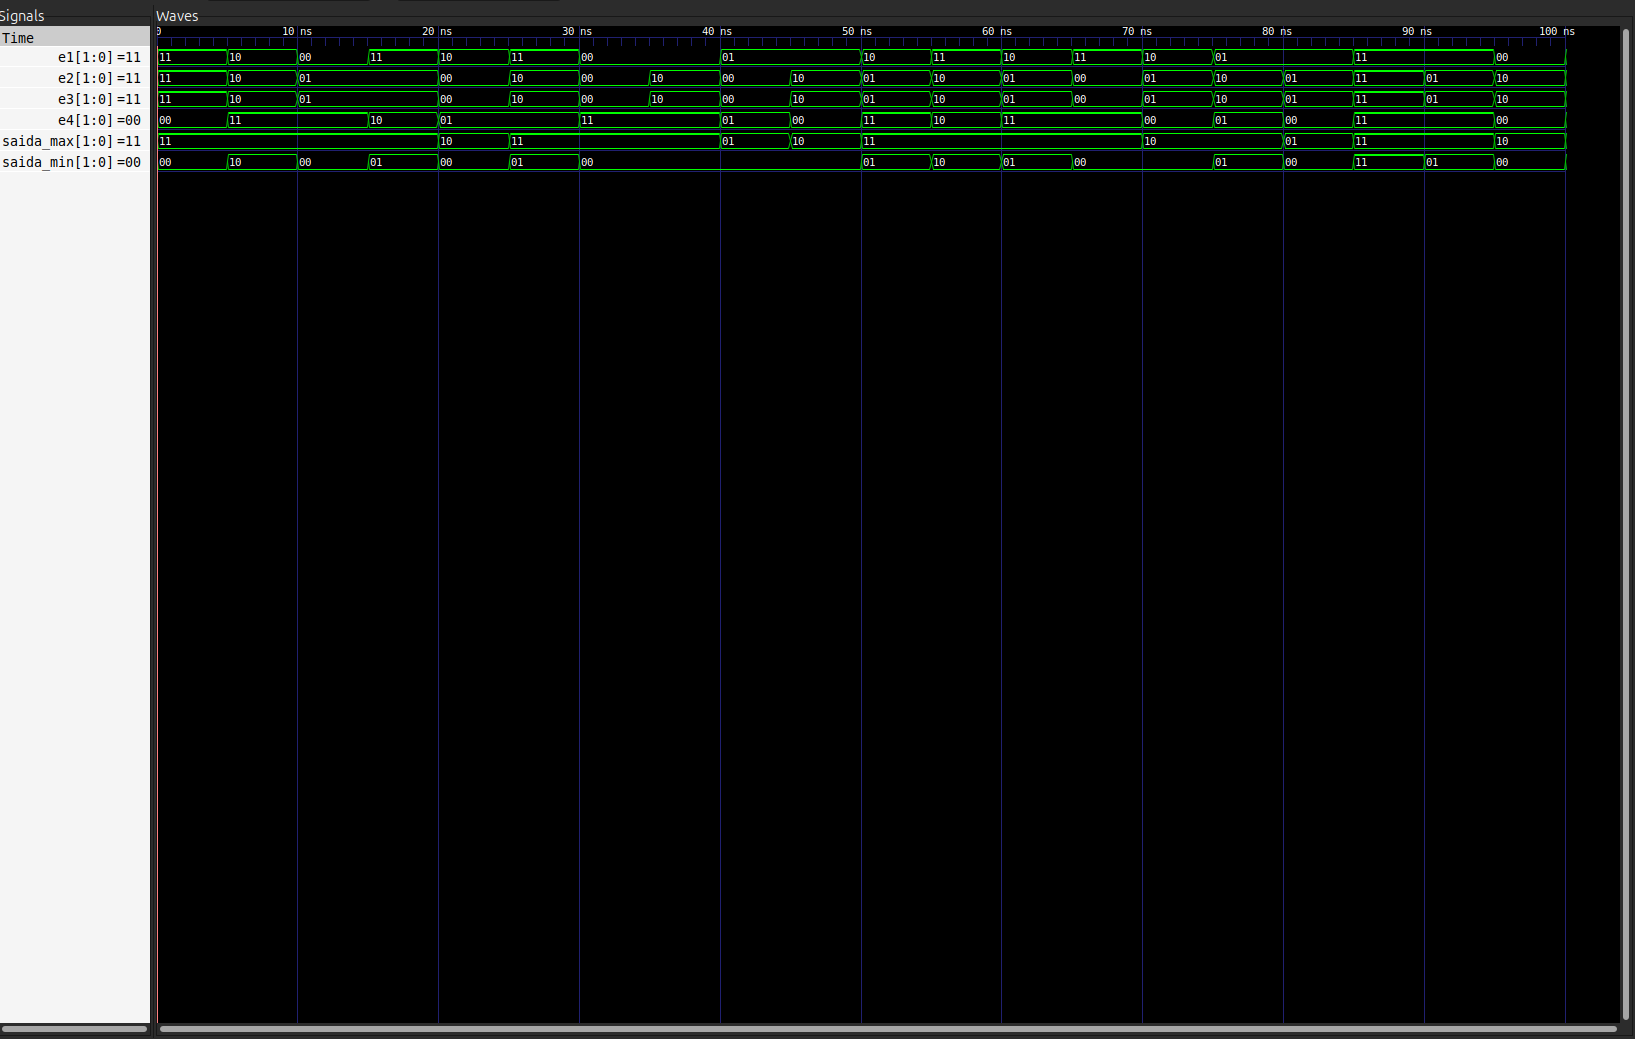
\includegraphics[width=0.95\textwidth]{simulacao.png}
    \caption{Formas de onda da simulação do detector de valor mínimo e máximo.}
    \label{fig:simulacao}
\end{figure}
\FloatBarrier

% ============================================================
\section{Diagrama RTL}
% ============================================================

O diagrama RTL gerado pelo Quartus Prime representa a entidade \texttt{atividade6} e a lógica combinacional responsável pela comparação dos valores de entrada. A estrutura sintetizada recebe os quatro valores convertidos para o vetor interno e produz os sinais de menor e maior valor, correspondentes às saídas \texttt{saida\_min} e \texttt{saida\_max}.

\begin{figure}[H]
    \centering
    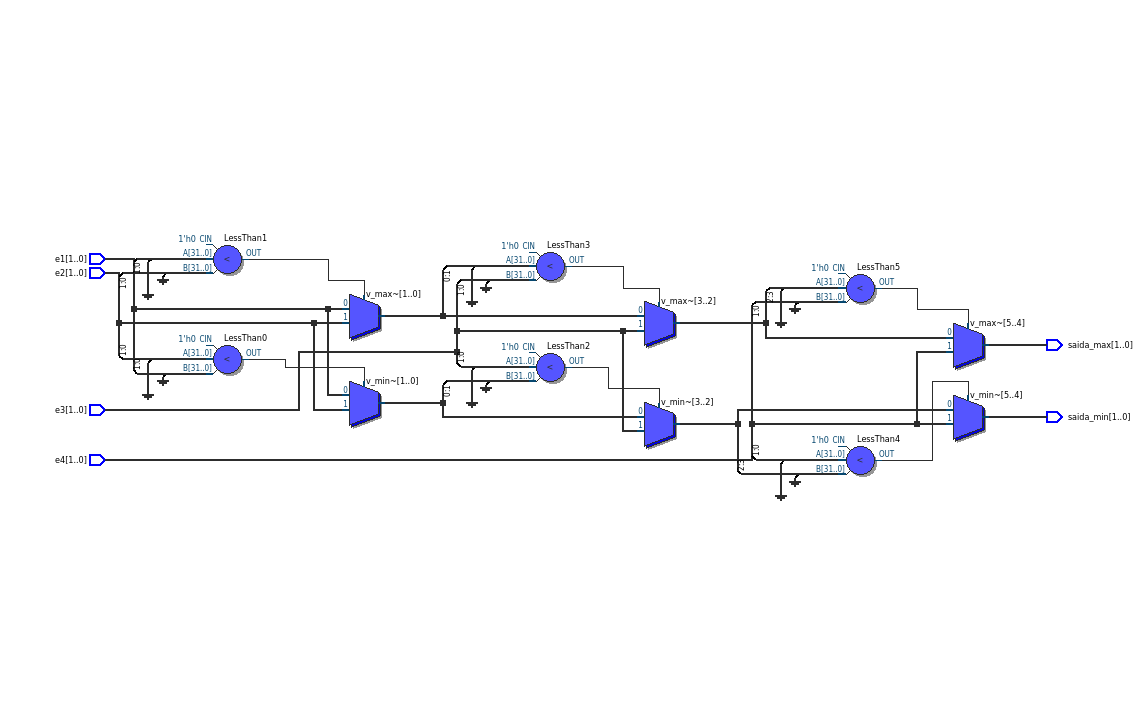
\includegraphics[width=0.95\textwidth]{RTL.png}
    \caption{Diagrama RTL do detector de valor mínimo e máximo.}
    \label{fig:rtl}
\end{figure}
\FloatBarrier

% ============================================================
\section{Considerações Finais}
% ============================================================

A atividade permitiu implementar um detector de mínimo e máximo utilizando \texttt{package}, \texttt{type}, \texttt{procedure} e \texttt{generic}. O pacote separa as declarações auxiliares da entidade principal, enquanto o procedimento concentra a lógica de comparação. A solução recebe quatro valores de 2 bits, converte-os para um vetor interno de inteiros, calcula os extremos e retorna os resultados nas saídas. A simulação confirmou o comportamento esperado e a atribuição de pinos possibilitou a implementação do circuito na placa DE10-Lite, utilizando chaves para as entradas e LEDs para a indicação dos valores mínimo e máximo.

% ============================================================
\appendix
% ============================================================

\newpage
\section{Código VHDL -- Pacote \texttt{meupacote}}
\label{ap:codigo-pacote}

\begin{lstlisting}[style=vhdl, caption={Arquivo \texttt{meupacote.vhd}.}]
library ieee;
use ieee.std_logic_1164.all;
use ieee.numeric_std.all;

package meupacote is
    -- Definição de tipo array de std_logic_vector conforme pedido
    type slv_array is array (natural range <>) of unsigned;
    
    -- Definição de tipo array de integer conforme pedido
    type int_array is array (natural range <>) of integer;

    -- Procedimento para encontrar min e max em um array de inteiros
    procedure detector_min_max (
        signal entrada : in  int_array;
        signal min_val : out integer;
        signal max_val : out integer
    );
end package meupacote;

package body meupacote is
    procedure detector_min_max (
        signal entrada : in  int_array;
        signal min_val : out integer;
        signal max_val : out integer
    ) is
        variable v_min : integer;
        variable v_max : integer;
    begin
        -- Inicializa com o primeiro elemento
        v_min := entrada(entrada'low);
        v_max := entrada(entrada'low);
        
        -- Loop para percorrer o array e comparar valores
        for i in entrada'range loop
            if entrada(i) < v_min then
                v_min := entrada(i);
            end if;
            if entrada(i) > v_max then
                v_max := entrada(i);
            end if;
        end loop;
        
        -- Atribui os resultados das variáveis aos sinais de saída
        min_val <= v_min;
        max_val <= v_max;
    end procedure;
end package body meupacote;
\end{lstlisting}

\newpage
\section{Código VHDL -- Entidade \texttt{atividade6}}
\label{ap:codigo-top}

\begin{lstlisting}[style=vhdl, caption={Arquivo \texttt{atividade6.vhd}.}]
library ieee;
use ieee.std_logic_1164.all;
use ieee.numeric_std.all;
use work.meupacote.all; -- Importando o pacote

entity atividade6 is
    generic (
        NUM_INPUTS : integer := 4; -- Quantidade genérica de valores
        NUM_BITS   : integer := 2  -- Quantidade genérica de bits (2 p/ caber nos 10 SW da DE10-Lite)
    );
    port (
        -- Interface em std_logic_vector para compatibilidade com o VWF
        e1, e2, e3, e4 : in  std_logic_vector(NUM_BITS-1 downto 0);
        -- Saídas de valor mínimo e máximo
        saida_min      : out std_logic_vector(NUM_BITS-1 downto 0);
        saida_max      : out std_logic_vector(NUM_BITS-1 downto 0)
    );
end entity;

architecture comportamento of atividade6 is
    -- Sinal interno utilizando o tipo definido no package
    signal x : int_array(0 to NUM_INPUTS-1);
    signal m_val, M_val_int : integer;
begin
    -- Mapeamento das portas std_logic_vector para o vetor de inteiros
    x(0) <= to_integer(unsigned(e1));
    x(1) <= to_integer(unsigned(e2));
    x(2) <= to_integer(unsigned(e3));
    x(3) <= to_integer(unsigned(e4));

    -- O process e uma instrucao concorrente da arquitetura.
    -- Dentro dele, a chamada do procedure e sequencial e recalcula min/max quando x muda.
    process(x)
    begin
        detector_min_max(x, m_val, M_val_int);
    end process;

    -- Converte os inteiros para std_logic_vector nas saídas
    saida_min <= std_logic_vector(to_unsigned(m_val, NUM_BITS));
    saida_max <= std_logic_vector(to_unsigned(M_val_int, NUM_BITS));

end architecture;
\end{lstlisting}

\end{document}
